\documentclass{article}
\usepackage{graphicx}

\usepackage[english]{babel}

\begin{document}

cloud data
 \begin{table}
 \small
 \begin{tabular}{|c|c|c|c|c|c|} 
 \hline 
Case & Read File  & Threads & \# of   & $T_C$ \\
& Size  (MB)&  per Task&  Tasks &  (seconds)  \\  \hline
s1 & 800 &  8 & 1 &366  \\
s2 & 400  & 4 & 2 &569  \\
s3 & 200 & 2 & 4 & 921  \\ 
s4& 100 & 1 & 8& 2001 \\
 \hline
 \end{tabular}
 \caption{With  Human Genome 18 Chromosome 21 10 index files   }
  %  \label{table:understandio}
\end{table}

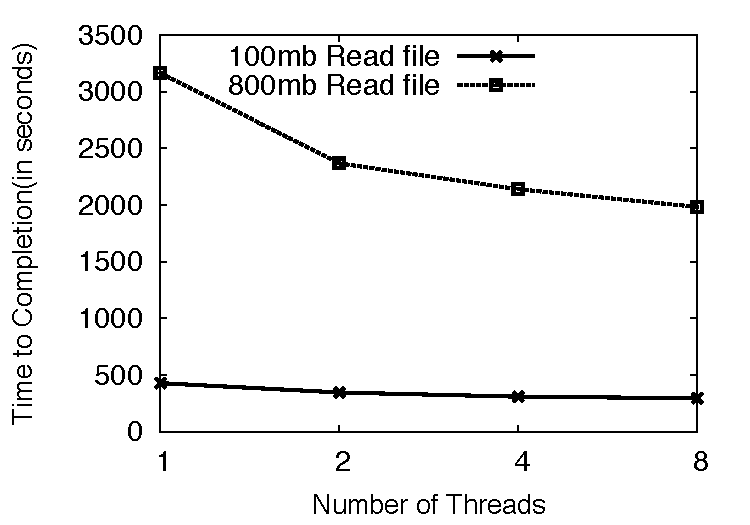
\includegraphics[scale=0.66]{../figures/cloud_threadsvstime.pdf} 



\end{document}

